\section*{Ejercicio 2}
\graphicspath{{Figuras/}}

Se busco estudiar una generalización del problemas de XOR para $N$ entradas, en donde la salida esperada es el producto de todas las componentes de la entrada. La arquitectura utilizada consistió en una capa oculta de $N'$ neuronas con una función de activación \texttt{tanh}, seguida de una capa de salida de 1 neurona tambien con activacion \texttt{tanh}. Debido a que la cantidad de datos de entrada es igual a $2^{N}$ y era de interés estudiar los casos en donde $N>N'$ y $N<N'$, se fijo $N$ a un valor de 5 y se entreno la red para distintos valores de $N'$: 1, 3, 5, 7, 9 y 11, en todos ellos durante 5000 épocas.

\begin{figure}[h!]
    \centering
    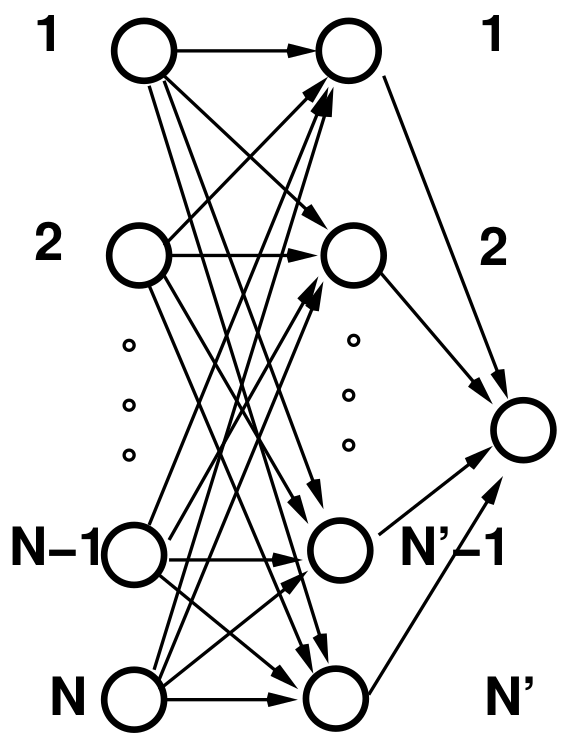
\includegraphics[width=0.3\textwidth]{Figuras/ejer_2_NN1.png}
    \caption{Esquema de la arquitectura utilizada para resolver el problema del XOR generalizado.}
    \label{02:fig:Arquitectura}
\end{figure}

En la Figura \ref{fig:2_Resultados} se observan los resultados obtenidos para la función de costo y \textit{accuracy} en cada uno de los casos. En caso de que $N'>N$, los resultados son similares a los del ejercicio anterior, ya que en una pequeña cantidad de épocas se obtiene un 100\% de precisión. La situación se vuelve mas problemática al disminuir $N'$, en donde se observa que para $N'=N=5$ el aprendizaje de la red nunca alcanza una precisión total e incluso no mejora de manera monótona conforme avanzan las épocas. Los resultados son incluso peores cuando $N'<N$, en donde se requieren muchas mas épocas para que la red aprenda e incluso para $N'=1$ nunca se logra alcanzar un valor de \textit{accuracy} no nulo. Este problema es esperable, ya que el valor de $N'$ determina las dimensiones de las matrices de pesos de cada una de las capas. Al disminuir $N'$, menor sera la cantidad de componentes de estas matrices, con lo cual deberá ajustar una gran cantidad de datos de entrada ($2^{N}$) con menos grados de libertad, que, en caso de ser demasiado pocos, se presentara un problema de underfitting y la red no mejorara sus resultados.


\begin{figure}[h!]
    \centering
    \begin{subfigure}[h]{0.49\textwidth} 
        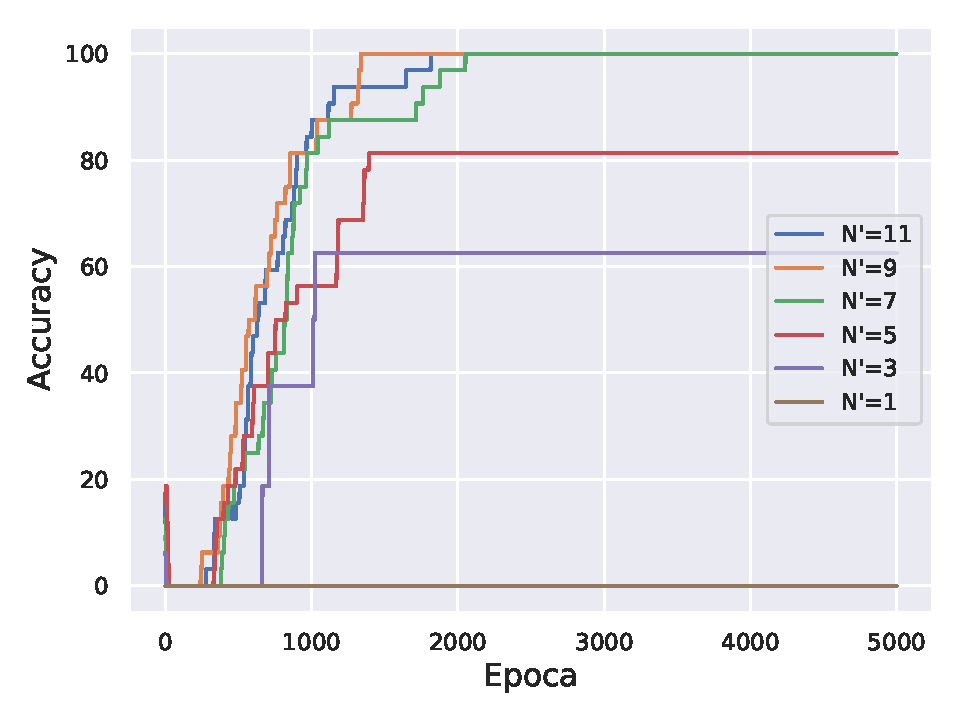
\includegraphics[width=\textwidth]{Figuras/ej2/Acc.pdf}
    \end{subfigure}       
    \begin{subfigure}[h]{0.49\textwidth} 
        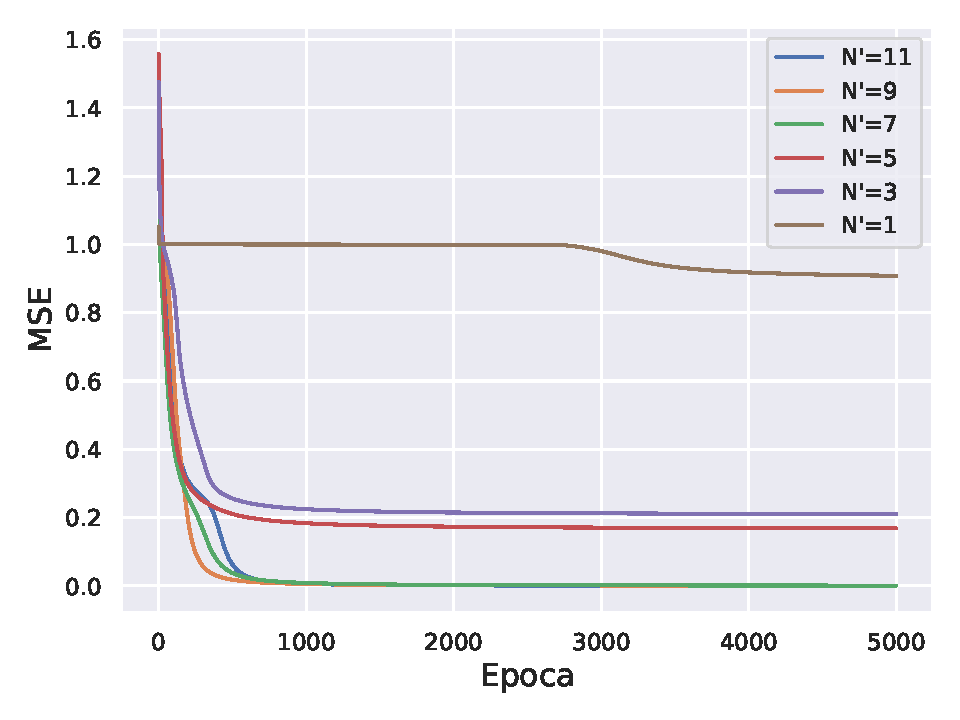
\includegraphics[width=\textwidth]{Figuras/ej2/Loss.pdf}
    \end{subfigure}
    \caption{Función de costo MSE y \textit{accuracy} para el entrenamiento de 6 modelos independientes variando la cantidad de neuronas de la capa oculta, utilizando la arquitectura propuesta en Fig. \ref{fig:1_Arquitecturas}.}
    \label{fig:2_Resultados}
\end{figure}